%---------------------------------------------------------------------
%
%                          Cap�tulo 4
%
%---------------------------------------------------------------------
%
% 04Imagenes.tex
% Copyright 2009 Marco Antonio Gomez-Martin, Pedro Pablo Gomez-Martin
%
% This file belongs to the TeXiS manual, a LaTeX template for writting
% Thesis and other documents. The complete last TeXiS package can
% be obtained from http://gaia.fdi.ucm.es/projects/texis/
%
% Although the TeXiS template itself is distributed under the 
% conditions of the LaTeX Project Public License
% (http://www.latex-project.org/lppl.txt), the manual content
% uses the CC-BY-SA license that stays that you are free:
%
%    - to share & to copy, distribute and transmit the work
%    - to remix and to adapt the work
%
% under the following conditions:
%
%    - Attribution: you must attribute the work in the manner
%      specified by the author or licensor (but not in any way that
%      suggests that they endorse you or your use of the work).
%    - Share Alike: if you alter, transform, or build upon this
%      work, you may distribute the resulting work only under the
%      same, similar or a compatible license.
%
% The complete license is available in
% http://creativecommons.org/licenses/by-sa/3.0/legalcode
%
%---------------------------------------------------------------------

\chapter{Implementaci\'on de las aplicaciones}
\label{cap4}
\label{cap:impl}

En este cap\'itulo se cubre todo el proceso de creaci\'on y desarrollo de las diferentes aplicaciones y la demo que posteriormente se utiliza como ejemplo de implementaci\'on de la herramienta.
Se ha divido este cap\'itulo en 3 apartados principales:

\begin {itemize}
\item Implementaci\'on de la aplicaci\'on de Android.
\item Implementaci\'on de la aplicaci\'on de Unity.
\item Inclusi\'on de la herramienta en un juego cerrado.
\end {itemize}

%-------------------------------------------------------------------
\section{Implementaci\'on de la aplicaci\'on de Android}
%-------------------------------------------------------------------

Este proyecto se ha desarrollado utilizando principalmente 2 tecnolog\'ias: Unity y Android Studio. Al tratarse de un proyecto de creaci\'on de un controlador para videojuegos y tomando como base la especificaci\'on desarrollada en el cap\'itulo 3 se ha optado por el desarrollo de una aplicaci\'on para Android que sirva como dispositivo de entrada y una aplicaci\'on en Unity que sirva como ejecutor del juego.

Android Studio es el entorno de desarrollo integrado (IDE) oficial para la plataforma de Android. Hasta finales del 2014 para desarrollar en Android se utilizaba Eclipse como IDE oficial y est\'a disponible para las plataformas Microsoft Windows, macOS y GNU/Linux. Android Studio incluye una gran variedad de herramientas para facilitar el desarrollo en Android entre las que se incluyen:

\begin {itemize}
\item Plantillas para crear dise\~nos comunes de Android y otros componentes.
\item Un editor de dise\~no enriquecido que permite a los usuarios arrastrar y soltar componentes de la interfaz de usuario.
\item Soporte para construcci\'on basada en Gradle.
\item Un dispositivo virtual de Android que se utiliza para ejecutar y probar aplicaciones.
\item Consola de desarrollador: consejos de optimizaci\'on, ayuda para la traducci\'on y estad\'isticas de uso.
\item Integraci\'on de ProGuard y funciones de firma de aplicaciones.
\end {itemize}
 
Los lenguajes de programaci\'on aceptados por Android Studio son Kotlin, Java y C++. En concreto para este proyecto se ha usado Java como lenguaje de programaci\'on.

%-------------------------------------------------------------------
\subsection {Ciclo de vida de Android}
%-------------------------------------------------------------------

Las aplicaciones en Android se rigen por una serie de componentes que se llaman \textbf{\textit{Activity}}. Estos componentes son claves a la hora de manejar los estados de una aplicaci\'on en Android. A diferencia de otros paradigmas de programaci\'on que comienzan sus aplicaciones con un m\'etodo \textbf{\textit{main()}}, la instancia de una Actividad invoca m\'etodos de devoluci\'on de llamada que se corresponden con etapas espec\'ificas de su ciclo de vida. La experiencia de una aplicaci\'on para un dispositivo m\'ovil difiere mucho de la versi\'on de escritorio de esa misma aplicaci\'on ya que la interacci\'on del usuario con la aplicaci\'on no siempre comienza en el mismo lugar. Un claro ejemplo de esto sucede con las aplicaciones de mensajer\'ia instantanea. Un usuario puede estar navegando por cualquier red social y encontrarse una publicaci\'on interesante y compartirla por correo electr\'onico o por una aplicaci\'on de mensajer\'ia instantanea. La aplicaci\'on de correo electr\'onico no se abre en el mismo estado si se abre desde la opci\'on de compartir de la red social o si se abre desde el men\'u de aplicaciones instaladas en el dispositivo. Las Actividades est\'an dise\~nadas para facilitar este paradigma.

La mayor\'ia de las aplicaciones contienen varias pantallas, lo cual significa que contienen varias actividades. Este concepto se pondr\'a posteriormente de manifiesto ya que para el desarrollo de la aplicaci\'on han sido necesarias 2 Actividades. Una actividad proporciona una ventana en la que la aplicaci\'on dibuja la interfaz de usuario. Esta ventana puede estar a pantalla completa o puede ser m\'as peque\~na y flotar sobre otras ventanas como si fuese un \textit{pop-up}.

Cuando un usuario navega por una aplicaci\'on, la cierra, la vuelve a abrir o la minimiza, las instancias de las Actividades de la aplicaci\'on pasan por una serie de estados de su ciclo de vida. Estos estados pueden tener comportamientos definidos por los desarrolladores de la aplicaci\'on. Esto permite tener un control sobre lo que ocurre en cada uno de los estados de la aplicaci\'on. Para navegar por las transiciones entre las etapas del ciclo de vida de una actividad, la clase Activity proporciona un conjunto b\'asico de seis devoluciones de llamadas: \textbf{onCreate() ,onStart(), onResume(), onPause(), onStop() y onDestroy().} El sistema invoca cada una de estas devoluciones de llamada cuando una operaci\'on entra en un nuevo estado.


\begin{figure}[h]
\caption{Ciclo de vida de una Actividad de un sistema Android}
\centering
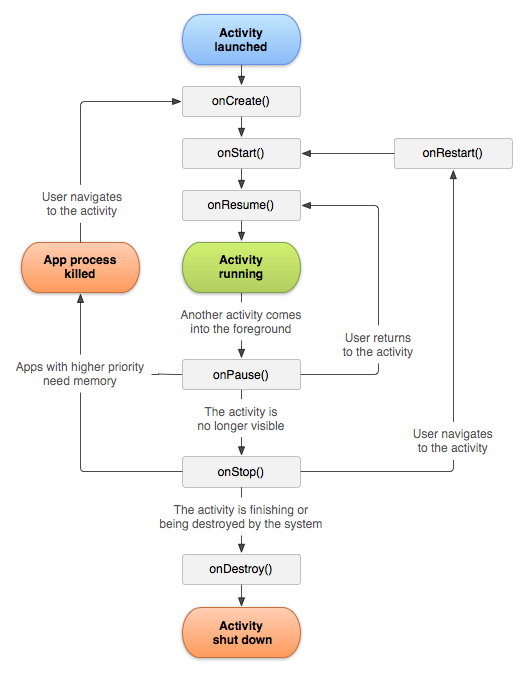
\includegraphics[width=0.7\textwidth]{./Imagenes/Bitmap/Ciclo_de_vida_Android}
\end{figure}

Cada uno de los estados que tiene la actividad es llamado en un momento concreto de la ejecuci\'on de la Actividad. Las caracter\'isticas de cada uno de estos estados son las siguientes:

\begin {itemize}
\item \textbf{onCreate()} $\rightarrow$ Este m\'etodo es el primero que llama cuando se crea la Actividad. Este estado es utilizado para ejecutar la l\'ogica de la aplicaci\'on que debe ocurrir \'unicamente una vez en todo el ciclo de vida. Este m\'etodo recibe el par\'ametro \textit{\textbf{savedInstanceState}}, que es un objeto de tipo \textbf{\textit{Bundle}} que contiene el estado ya guardado de la actividad. Si la actividad nunca existi\'o, el valor del objeto \textit{Bundle} es nulo.
\item \textbf{onStart()} $\rightarrow$ 
\end {itemize}

%-------------------------------------------------------------------
\section{Android}
%-------------------------------------------------------------------

\begin {itemize}
\item Explicaci\'on muy despacito de qu\'e es un ciclo de vida. Hablar sobre Actividades y los estados que tienen estas Actividades.
\item Explciaci\'on de niveles de API y permisos. La aplicaci\'on est\'a preparada para leer un c\'odigo QR si o si en el formato IP:Puerto. Todo esto hace que mencione el QR al hablar de Android, seria recomendable hacer una subseccion para hablar del uso del QR, "historia" de este tipo de c\'odigos, etc?
\item Veis mejor hacer aqui una subseccion para explicar arquitectura y otra para explicacion del uso?
\item Subseccion dedicada unicamente a la concurrencia y comunicacion entre hilos.
\item subseccion para la arquitectura?
\end {itemize}


%-------------------------------------------------------------------
\section{Unity}
%-------------------------------------------------------------------

\begin {itemize}
\item Uso de Unity (entidades, ciclo de vida de entidades, lenguaje de scripting usando .NET)
\item Usos habituales del QR aqui? Mejor hacerlo en el apartado de Android?
\item Uso de las hebras para el tratamiento de los datos que se leen desde la hebra de red que tenemos pendiente de la llegada de datos al socket.
\item Uso de una hebra para mandar datos por la red.
\item Subseccion para explicar la utilizacion de esto?
\item subseccion para la arquitectura?
\end {itemize}


% Variable local para emacs, para  que encuentre el fichero maestro de
% compilaci�n y funcionen mejor algunas teclas r�pidas de AucTeX
%%%
%%% Local Variables:
%%% mode: latex
%%% TeX-master: "../ManualTeXiS.tex"
%%% End:
